\documentclass[11pt]{article}
\usepackage{amssymb}
\usepackage{amsmath}
\usepackage[usenames,dvipsnames]{xcolor}
\usepackage{indentfirst}
\usepackage{microtype}
\usepackage[a4paper, total={170mm,257mm}, left=20mm, top=20mm]{geometry}
\usepackage[symbol]{footmisc}
\usepackage{subfigure}
\usepackage{graphicx}
\usepackage{enumerate}

\renewcommand{\thefigure}{\arabic{label}}

\renewcommand{\thefootnote}{\fnsymbol{footnote}}


\setcounter{section}{-1}
	
\renewcommand*\contentsname{Tartalomjegyzék}

\AddToHook{cmd/section/before}{\clearpage}

\begin{document}
\begin{titlepage}
	\centering \vfill
	{\textsc{Budapesti Műszaki és Gazdaságtudományi Egyetem} \par} \vspace{7cm}
	{\huge\bfseries Elektornikai Technológia és Anyagismeret\par} \vspace{0.5cm}
	{\large \textsc{Előadások anyagát összefoglaló jegyzet}\par} \vspace{1.5cm}
	{\Large\itshape Készítette: Illyés Dávid\par} \vfill

	\noindent\fbox{%
    	\parbox{140mm}{
			\color{red}\textbf{Ez  a jegyzet nagyon hasonlóan van struktúrálva az előadás jegyzetekhez és fő célja, hogy olyan módon adja át a "A Programozás Alapjai 1" nevű tárgy anyagát, hogy az teljesen kezdők számára is könnyen megérthető és megtanulható legyen. }
   		}
	}
	
	\vfill {\large \today\par}
\end{titlepage} 
\tableofcontents
\addtocontents{toc}{~\hfill\textbf{Oldal}\par}

    \section{0 Bevezetés, fogalmi rendszerezés}

        \paragraph{Mi az Elektronikai Technológia?} A technológia az anyag jellemzőinek tervezett, maradandó megváltoztatása. Az elektronikai texhnológia a villamosmérnöki tudományos és Ipari-kereskedelemi ismereteknek azon területe, amely az elektronikus áramköri egységek alkatrészeinek, hordotóinak és összeköttetés rendszereinek tervezésével, megvalósításával és megbízhatóságával foglalkozik.

		\paragraph{Az elektronikai technológia hatóereje.} A funkciók integrációja a méret, az energiafelhasználás, a költségek és a környezeti terhelés optimalizálása, tervezhető megbízhatóság mellett.

		\paragraph{Mi az anyagismeret célja?}

			\begin{itemize}
				\item Az ipar különböző területein alkalmazható anyagok (természetes és szintetikus polimerek, fémek és ötvözeteik, egykristályos, kerámikus anyagok és kompozitok) felépítésének, fizikai, technológiai és használati jellemzőinek rendszerezése.
				\item Az anyagkiválasztás szempontrendszerének és módszertanának összefoglalása.
			\end{itemize}

		\paragraph{Mivel foglalkozik a tárgy?} 

			\begin{itemize}
				\item Elektronikus készülékek konstrukciós alapelvei, megbízhatóság és termikus tervezés.
			\end{itemize}

	\section{1 Elektronikus készülékek}

		\subsection{Készülékek fejlesztési fázisai}

			\begin{enumerate}
				\item Műszaki specifikáció meghatározása (50\%\footnote[1]{:a termék sikerességében való szerep aránya}):
					\begin{itemize}
						\item Egyeztetés, marketing, bench-marking, meglévő és várható előírások, hatósági előírások.
					\end{itemize}
				\item Prototípus kifejlesztése (30\%\footnotemark[1]):
				\begin{itemize}
					\item Specifikáció, tesztelés, gyárthatósag, ár.
				\end{itemize} 
				\item Gyártástechnológia kidolozása (10\%\footnotemark[1])
				\begin{itemize}
					\item Gyártási költségek, gyártáskapacitás, tesztelés.
				\end{itemize}
				\item Próbagyártás (10\%\footnotemark[1])
				\begin{itemize}
					\item Tesztelés (kihozatal/selejt arány).
				\end{itemize} 
				\item Gyártás (0\%\footnotemark[1])
				\begin{itemize}
					\item Minőségellenőrzés, SPC.
				\end{itemize}
			\end{enumerate}

		\subsection{Út a műszaki specifikációig}
			
			\subsubsection{Mit kell létrhozni?}

				A mérnöki gyakorlatban olyan készülékekkel foglalkozunk, amelyekre \underline{igény} mutatkozik.

				Az igény lehet:

				\begin{itemize}
					\item valós:
					\begin{itemize}
						\item item egyedi (pl. atomerőmű),
						\item nem egyedi, vagy piaci (pl. autó), 
					\end{itemize}
					\item látens (pl. SMS),
					\item a kitalálás pillanatában még nem létező (pl. Rubik Kocka)
				\end{itemize}

			\subsubsection{Ki lesz a felhasználó? (jelen és jövő)}

				\begin{itemize}
					\item Gyerek, felnőtt (férfi vagy nő),
					\item idős/beteg,
					\item átlagos fogyasztó,
					\item szakember,
					\item specialista.
					\begin{itemize}
						\item $\rightarrow$ \textcolor{red}{funkciók, ergonómiai szempontok}
					\end{itemize}
				\end{itemize}

			\subsubsection{Hol használjuk? (jelen és jövő)}

				\begin{itemize}
					\item Beltér/kültér, hideg/meleg (konyha, fürdőszoba),
					\item strandon, víz alatt, 20000 m magasan, 
					\item kemencében, váltóban (forró olajban), kipufogócsőben,
					\item műholdon.
						\subitem $\rightarrow$ \textcolor{red}{a működési környezet feltételi} (T, RH, p stb.)
				\end{itemize}

			\subsubsection{Mikorra kell elkészíteni? Mennyire szigorú a határidő?}

				\begin{itemize}
					\item A piaci megjelenés időpontjának optimuma van:
					\begin{itemize}
						\item hosszabb fejlesztési idő alatt a készülék tulajdonságaival lehet megelőzni a konkurenciát,
						\item gyor piaci megjelenéssel a készülék újdonságereje nagyobb,
					\end{itemize}
					\item egyéb szempontokat figylemen kívül hagyva, a piaci megjelenés idejének csökkentésével a kültségek meredeken növekszenek,
					\item a határidő betartása:
					\begin{itemize}
						\item az esetek többségében fontos, de csúszás tolerálható
						\item  egyes esetekben kulcsfontosságú (pl. Spirit Rover)
					\end{itemize}
				\end{itemize}

			\subsubsection{Mennyibe fog kerülni a készülék?}

				Pontosabban megfogalmazva: \textbf{gazdaságos}-e a készülék kifejlesztése, előállítása, gyártása? Mennyibe fog kerülni a piacra dobásig? Az előzetes költségbecslés a tervet még a megszületése előtt keresztbehúzhatja. Hiába jó (és megvalósítható, eladható, stb.) egy ötlet, ha a gyártó számára nem gazdaságos a megvalósítás.

				A költségek fontosabb összetevői:

				\begin{itemize}
					\item fejlesztés,
					\item gyártástervezés, gyártósor felállítása,
					\item gyártás,
					\item utóélet,
					\begin{itemize}
						\item (üzemeltetés),
						\item terméktámogatás (alkatrész utánpótlás),
						\item karbantartás,
						\item garanciális problémák kezelése,
						\item újrahasznosítás.
					\end{itemize}				
				\end{itemize}

			\subsubsection{További kérdések}

				(sokszor már ezen a szinten pontosan kell választ adni)

				\begin{itemize}
					\item a készülék tervezett és megvalósítható térfogatigénye, tömege,
					\item a készülék energiaigénye, 
					\item tervezett élettertam,
					\item megfelelés a szabányoknak és direktíváknak.
				\end{itemize}

				Elkerülhette valami a figyelmünket a stratégiai kérdésekben?

				Komplex fejelsztési projektekben \textbf{\underline{megvalósíthatósági tanulámnyt}} kell készíteni.

			\textbf{\textcolor{red}{IDE JÖN A 8. OLDALON LÉVŐ ÁBRA}}

		\subsection{Az áramkör tervezés célja}
			
			Az áramkörtervezés fő célja, hogy az áramköri hordozót és a passzív-aktív alkatrészek készletét felhasználva, \textbf{mérnöki szemléleti} előállítsunk egy áramkört.

			\underline{Megfelelő funkcionálítás főbb feltételei:}

			\begin{itemize}
				\item Alkatrészek értékei, tűrései, paraméterei;
				\item Felhasznált anyagok paraméterei, tűrései;
			\end{itemize}
			
			Példák:

			\begin{itemize}
				\item Hőmérséklet, tápfeszültség, villamos analóg és digitális paraméterek;
				\item Gyártási tolerancia (nem tőlünk függ - legfeljebb a gyártó megválasztásával);
				\item Dokumentáció - megfelelő- az alkatrész leírása a munka megkönnyítése érdekében?
			\end{itemize}
			
			Ezek szükségesek ahhoz, hogy összeálljon, tesztelhető legyen és megfelelően működjön a tervből előállított áramkör.

		\subsection{Áramkör tervezés - elektromos konstrukció}

			\begin{enumerate}
				\item Kapcsolási rajz készítés,
				\item részegységekre bontás, csatlakozó kiosztás,
				\item nyomtatott áramköri tervezés:
				\begin{itemize}
					\item számítógépes tervezőrendszerek (ORCAD, Pads...),
					\item alkatrész elrendezés (placer),
					\item összehuzalozás (router),
				\end{itemize}
				\item készülékhuzalozás.
			\end{enumerate}

		\subsection{Általános munkafolyamat}

			\textbf{\textcolor{red}{13 oldal ábra}}

			Iteratív folyat - egyes lépésekról visszatérhetünk korábbi pontokba! 
			
			Előre/hátra annotációnak hívják az ilyen megoldásokat.

			A terv különböző szintjeit a netlista file köti össze.

			Három részre különíthető a teljes EDA/ECAD folyamt a fogalmi rendszer szerint:

			\begin{itemize}
				\item Computer Aided Engineering (CAE)
				\item Computer Aided Design (CAD)
				\item Computer Aided Manufacuturing (CAM)
			\end{itemize}

		\subsection{Mechanikai tervezés, szerkezeti konstrukció}

			\begin{itemize}
				\item Készülk mechanikai vázszerkezetének tervezése,
				\item doboz és burkolat kialakítás - formatervezés,
				\item részegységek belső elrendezése:
				\begin{itemize}
					\item sínrendszer szerelés,
					\item alaplap,
					\item tövvkártyás rendszer,
				\end{itemize}
				\item előlap-, kezelőlap-, hátlaptervezés - ergonómia.
			\end{itemize}

		\subsection{Termikus tervezés}

			\begin{itemize}
				\item Különösen fontos nagy elemsűrűségű (laptop) és nagy teljesítményű (tápegység) készülékek esetén
				\item Szoftver eszközök:
				\begin{itemize}
					\item termikus szimuláció,
				\end{itemize}
				\item hardver eszközök:
				\begin{itemize}
					\item termikus interface,
					\item hűtőbordák,
					\item ventillátorok,
					\item heat pipe.
				\end{itemize}
			\end{itemize}

		\subsection{Elektromágneses zavarvédelmi tervezés}

			\textbf{\textcolor{red}{Esetleg ide is jöhet a kép a 16. oldalról}}

			\begin{itemize}
				\item EMC (elektromágneses kompatibilitás):
				\begin{itemize}
					\item a készülék által kibocsátott zavar megfelelően kicsi, 
					\item a készülék immunitása megfelelően nagy.
				\end{itemize}
				\item Zavarforrások:
				\begin{itemize}
					\item természetes:
					\begin{itemize}
						\item villámlás, elektromos energia kisülés,
						\item kozmikus sugárzás,
						\item naptevékenységgel kapcsolatos zavarok, 
						\item légkörből, ionoszférából érkező zavarok,
					\end{itemize}
					\item mesterséges:
					\begin{itemize}
						\item műsorszórók: rádió és TV adók,
						\item mobiltelefonok,
						\item rádiótelefonok,
						\item radarok,
						\item teljesítmény kapcsolók, relék,
						\item felvezetős teljesítményszabályzók,
						\item motorok, egyenirányítók.
					\end{itemize} 
				\end{itemize}
			\end{itemize}

		\subsection{Ergonómiai tervezés}

			\begin{itemize}
				\item Készülékek kezelés szempontjából történő optimális kialakítása - előlap, kezelőlap tervezés. Példa: elektronikus műszerek
				\begin{itemize}
					\item egyértelmű, esztétikus feliratozás,
					\item kijelzők és kezelőszervek működési elv szerinti összerendelése,
					\item összetartozó elemek egy csoportban, színnel jelölve, keretbe foglalva, 
					\item fontos kezelőszervek mellett LED indikátor, 
					\item nagyteljesítményű nyomógomb és kapcsoló - nagyobb méret,
					\item halózati főkapcsoló az előlap valamelyik szélén, 
					\item legfontosabb indikátor az előlap bal felső sarkában.
				\end{itemize}
			\item Optimális munkakörülmények, munkahelyek kialakítása. Példa: szerelő munkahely	
			\end{itemize}

		\subsection{Üzembiztonságra tervezés}
			
			\begin{itemize}
				\item Üzembiztonság fogalomköre:
				\begin{itemize}
					\item életvédelem, balesetvédelem, vagyonvédelem,
					\item rendeltetésszerű és meghibásodott állapotban sem okozhat kárt, veszélyt,
					\item az okozott kárért, balesetért a tervezp és gyártó a felelős!
					\item Safety Engineer.
				\end{itemize}
				\item Üzembiztonsági, környezetállósági témakörök:
				\begin{itemize}
					\item környezeti hatások elleni védelem:
					\begin{itemize}
						\item klimatikus, 
						\item kémiai, biológiai,
						\item mechanikai igénybevételek, autóiparban rezgések elleni védelem,
					\end{itemize}
					\item túláramvédelem,
					\item túlmelegedés elleni (tűz) védelem,
					\item káros szgárzások elleni védelem, 
					\item robbanásvédelem.
				\end{itemize}
			\end{itemize}

		\subsection{Érintésvédelmi tervezés}

			\begin{itemize}
				\item A készülékek fémes részei, amelyek üzemszerűen nincsenek feszültség alatt, meghibásodás esetén se okozhassanak áramütést. A szabványok betratása kötelező!
				\begin{itemize}
					\item \textbf{"0." Érintésvédelmi osztály:}
					\begin{itemize}
						\item Elkerítés, elszigetelés, burkolás - nincs érintésvédelemi kapocs.
					\end{itemize}
					\item \textbf{"I." Érintésvédelmi osztály:}
					\begin{itemize}
						\item Üzemi szigetelés + megérinthető fémrészek összekötve (pl. készülékház + ajtó) és a hálózati védőföldre kötve (védőeres hálózati kábel, színjelzés: zöld-sárga).
					\end{itemize}
					\item \textbf{"II." Érintésvédelmi osztály:}
					\begin{itemize}
						\item Szigetelőanyag burkolat: az összes fémrészt burkolja (pl. hajszárító). A külső burkolat egyben a védőszigetelés is.
					\end{itemize}
					\item \textbf{"III." Érintésvédelmi osztály:}
					\begin{itemize}
						\item Érintési feszültség 24 - 50 $V_{eff}$ AC
						\item Nincs olyan áramköri rész, amely ennél nagyobb feszültségen üzemel.
					\end{itemize}
				\end{itemize}
			\end{itemize}

			\textbf{\textcolor{red}{Ide 19. oldal ábrák és példák jöhetnek.}}

		\subsection{IP - Védelem kérdése (Ingression Protection)}

			\textbf{\textcolor{red}{20. oldali táblázat ide}}

		\subsection{Gyárthatóságra tervezés (DFM)}

			\begin{itemize}
				\item Minőségügy, 6 szigma,
				\item terméktervezés, amley figyelembe veszi a gyártási követelményeket, 
				\item olyan tervezési lépés, amelyben csoportmunkát alkalmazunk a termék kifejlesztésére,
				\item több eszközt és technikát magába foglaló keret a gyártható termék létrehozására.
			\end{itemize}

			\textbf{Előnyök:}

			\begin{itemize}
				\item alacsonyabb fejlesztési költség,
				\item rövidebb fejlesztési idő, 
				\item rövidebb idő a gyártás megkezdéséig,
				\item alacsonyabb szerelési és tesztelési költségek, 
				\item jobb minőség.
			\end{itemize}

		\subsection{Gyráthatóságra, tesztelhetőségre tervezés (DFM)}

			\textbf{Irányelvek:}

				\begin{itemize}
					\item minimalizáljuk az alkatrészek számát,
					\item használjuk a szabványos és azonos elemeket, 
					\item minimalizáljuk a szerelési síkok számát (Z-axis), 
					\item használjunk standerd szerszámfejeket, fúrókat, eszközöket,
					\item kerüljük a szűk furatokat (forgácsok, egyenesség, eltömődés), 
					\item használjuk a közös méretet a szerszámrögzítéshez,
					\item minimalizáljuk a szerlési irányokat,
					\item miximalizáljuk a hozzáférhetőséget; szerlésre tervezés,
					\item minimalizáljuk a kézi műveleteket,
					\item küszöböljük ki az utólagos állítást,
					\item használjuk ismételhető, jól ismert folyamatokat, 
					\item tervezzük az alkatelemeket a hatékony tesztelés lehetőségére,
					\item kerüljük a rejtett részleteket,
					\item hozzunk létre szimmetriát két irányban, 
					\item kerüljünk az összekuszálás lehetőségét, 
					\item tervezzünk önmegvezető (önpozicionáló) elemeket.
				\end{itemize}

		\subsection{Megbízhatósági tervezés}

			\begin{itemize}
				\item Soros struktúrájú (redundanciamentes) rendszer jellemzői: 
				\begin{itemize}
					\item a rendszer véges számú elemből áll, 
					\item egy elem meghibásodása a rendszer meghibásodásához vezet,
					\item a meghibásodások egymástól függetlenek, 
					\item a kommersz elektronikai berendezések soros struktúrájúak.
				\end{itemize}
				\item Melegtartalékolt (párhuzamos) rendszer jellemzői:
				\begin{itemize}
					\item a rendszer $n$ azonos elemből áll,
					\item a rendszer műkökéséhez egy elem működése szükséges, 
					\item hibafelismerő elem, kapcsolóelem esetenként szükséges,
					\item a tartalék állapota ismert, 
					\item a taralék is fogyaszt energiát, elhasználódik.
				\end{itemize}
				\item Hidegtartalékolt rendszer jellemzői:
				\begin{itemize}
					\item a rendszer $n$ azonos elemből áll, 
					\item a rendszer működéséhez egy elem működése szükséges, 
					\item a tartalékban lévő elem nincs bekapcsolva, nem fogyaszt energiát,
					\item a tartalékban lévő elem nem hibásodhat meg,
					\item hibafelismerő és kapcsolóelemre van szükség,
					\item a tartalékelem bakapcsolása időt vesz igénybe.
				\end{itemize}
			\end{itemize}

		\subsection{Szabvényokra épülő megvalósítás}

			Előnye:

			\begin{itemize}
				\item nem szükséges intuitív tervezés, 
				\item minden paraméter (méret, térfogategységre eső disszipáció, stb.) szabványokból kiválasztható,
				\item rejtett hibák felbukkanásának esélye kisebb.
			\end{itemize}

			Hátránya:

			\begin{itemize}
				\item a tervező keze teljesen kötött,
				\item egyedi ötletek megvalósítása nem lehetséges,
				\item a készülék az esetek döntő többségében jelentősen "túltervezett",
				\item nagyobb tételben a gyártás gazdaságtalanná válhat.
			\end{itemize}

		\subsection{Szabványokat részben követő megvalósítás}

			\begin{itemize}
				\item Ez a gyakoribb eset, 
				\item kötelező szabványok (EMC, érintés védelem, gép direktíva stb.) minden körülmények között betartandóak,
				\item lehetőseg van az ár/költség/kihozatal/gyrátási kapacitás optimalizálására,
				\item valamennyi tervezési fázis szükséges,
				\item lehetőség van minden paraméterben a folyamatos gyrátmány fejlesztésére,
				\item pélad: notebook konstrukció.
			\end{itemize}

	\section{2 Elektronikai szerelési- és kötéstechnológiák}

		\subsection{Az elektronikai alkatrészek csoportosítása}

			\begin{itemize}
				\item \textcolor{red}{Funkció szerint:}
					\subitem{aktív, passzív}
				\item \textcolor{red}{Szerelhetőség szerint:}
					\subitem furatszerelt, felületszerelt, tokozatlan chip
				\item \textcolor{red}{Funkciók száma szerint:}
					\subitem diszkrét alkatrészek - egy alkatrész egy áramköri elemet tartalmaz
					\subitem integrált áramkörök - egy alkatrész több áramköri elemt tartalmaz
			\end{itemize}

			\textbf{\textcolor{red}{2. oldali ábrák jöhetnek ide}}

		\subsection{A szerelt nyomtatott huzalozású lemez felépítése}

			\begin{figure}[!htb]%
				%% first three subfigures
				\subfigure[]{
					\label{fig:1}
					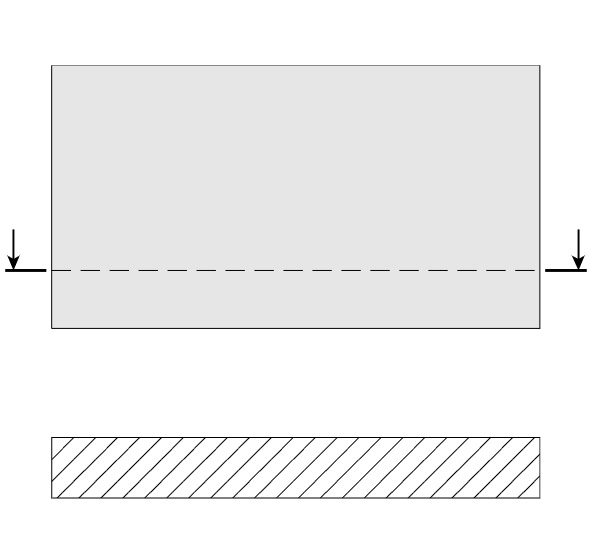
\includegraphics[width=0.31\textwidth]{images/2.2/1.jpg}%
				}%
				\hspace{\fill}
				\subfigure[]{ 
					\label{fig:2}
					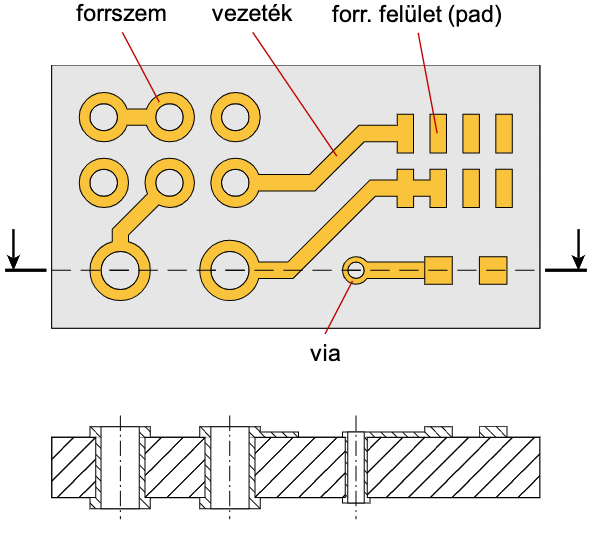
\includegraphics[width=0.31\textwidth]{images/2.2/2.png}%
				}%
				\hspace{\fill}
				\subfigure[]{
					\label{fig:3}
					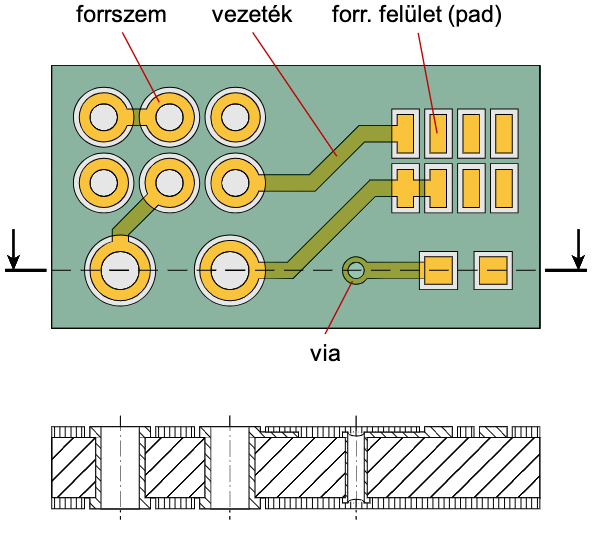
\includegraphics[width=0.31\textwidth]{images/2.2/3.png}%
				}
			
				%% second group of subfigures
				\subfigure[]{
					\label{fig:4}
					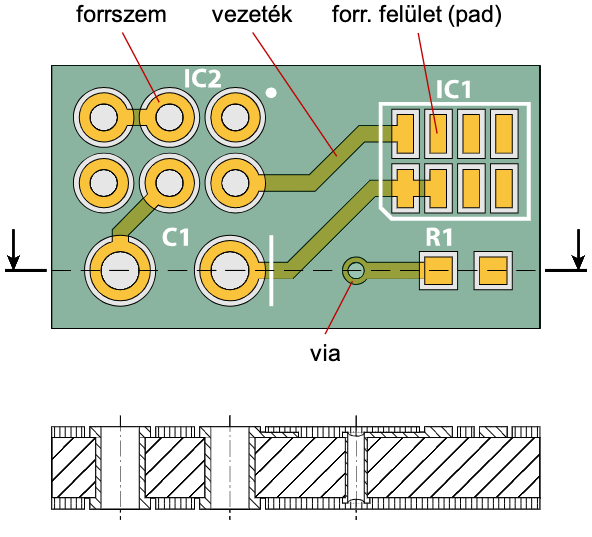
\includegraphics[width=0.31\textwidth]{images/2.2/4.png}%
				}%
				\hspace{\fill}
				\subfigure[]{
					\label{fig:5}
					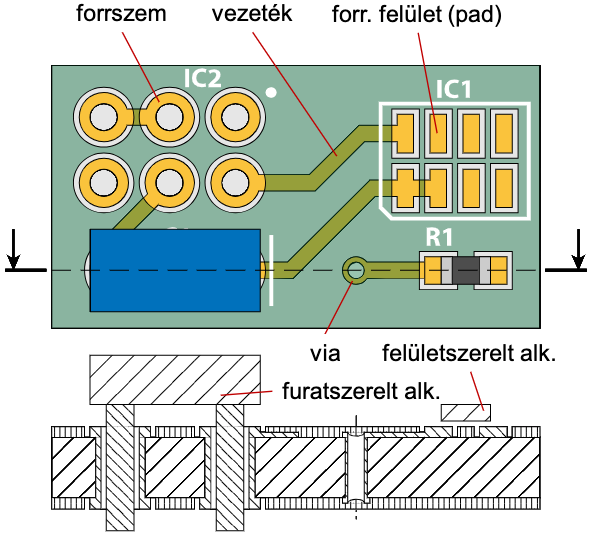
\includegraphics[width=0.31\textwidth]{images/2.2/5.png}%
				}%
				\hspace{\fill}
				\subfigure[]{
					\label{fig:6}
					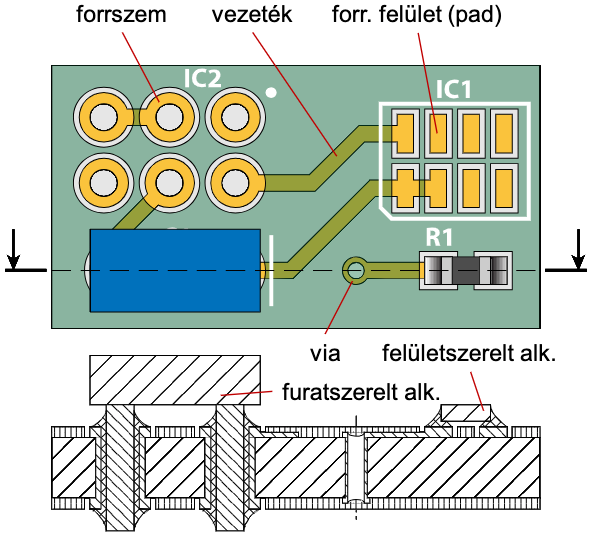
\includegraphics[width=0.31\textwidth]{images/2.2/6.png}%
				}
			\end{figure}

			\begin{enumerate}[a]
				\item Hordozó, pl. FR4 üvegszálas epoxigyanta
				\item Réz mintázat: fotolitográfiával kialakított
				\item Forrasztásgátló maszk: szitanyomtatással viszik fel és fotolitográfiával mintázzák
				\item Feliratok, pozícióábrák: szitanyomtatással viszik fel
				\item Alkatrészek beültetése: kézi, gépesített
				\item Forrasztás: hullámforrasztás, újraömlesztéses forrasztás
			\end{enumerate}

		\subsection{Furatszerelt alkatrészek}

			\begin{itemize}
				\item \textcolor{red}{Hajlékony} vagy \textcolor{red}{merev} kivezetésekkel (alaktrészlábakkal) rendelkeznek. A hajlékony kivezetéseket a furatok helyzetének megfelelően méretre vágják és hajlítják.
				\item A kivezetéseket a szerelőlemez furataiba illesztik és többnyire a másik oldalról forrasztják be. Ezért a csak furatszerellt alkatrészeket tartalmazó áramköröknél megkülönböztetünk \textcolor{red}{alkatrész-} és \textcolor{red}{forrasztási} oldalt.
			\end{itemize}

			\begin{center}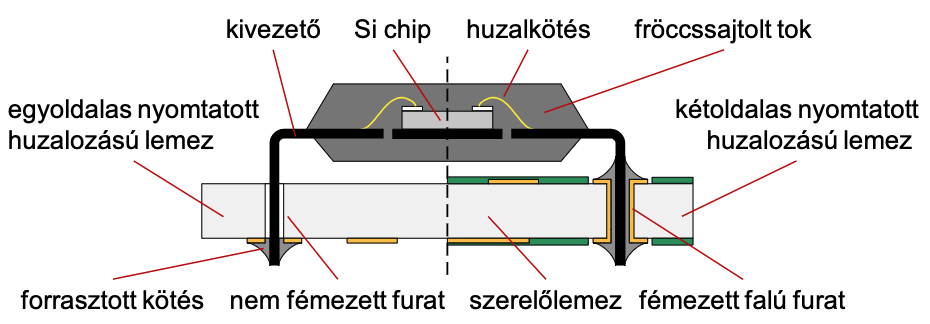
\includegraphics[width=0.75\textwidth]{images/2.3/1.png}\end{center}

		\subsection{Furatszerelt alkatrészek csoportosítása}

			\begin{center}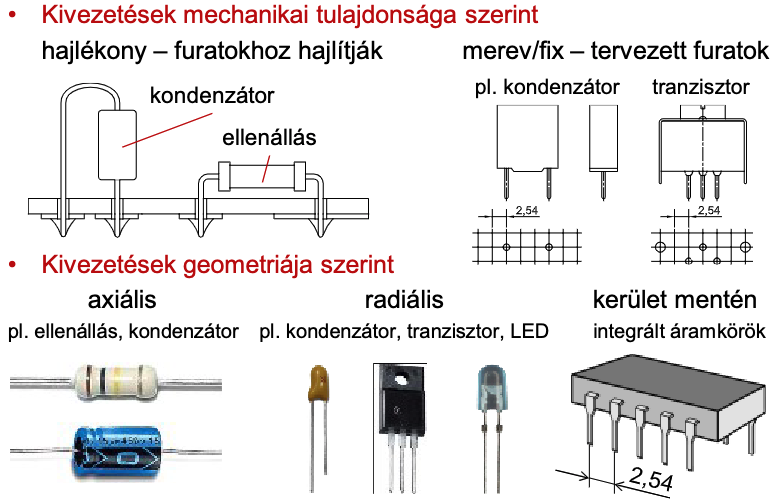
\includegraphics[width=.95\textwidth]{images/2.4/1.png}\end{center}

		\subsection{Diszkrét furatszerelt alkatrészek (Passzív)}

			\begin{center}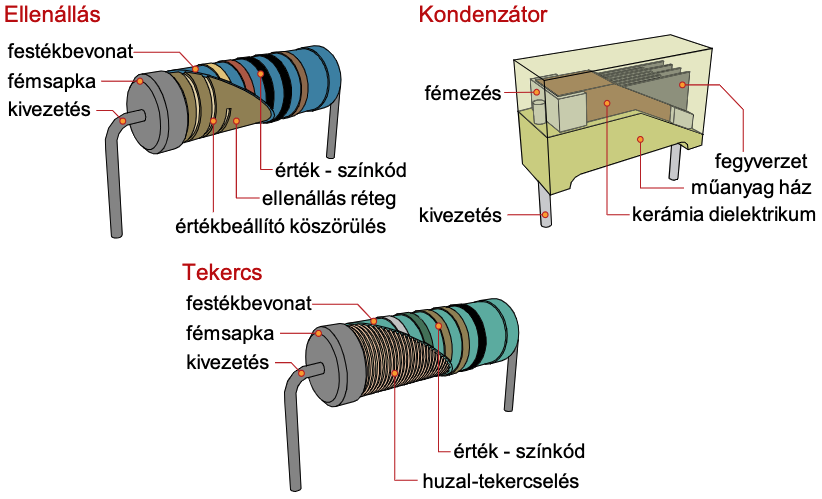
\includegraphics[width=.95\textwidth]{images/2.5/1.png}\end{center}

		\subsection{Furatszerelt aktív alkatrészek}

			\begin{center}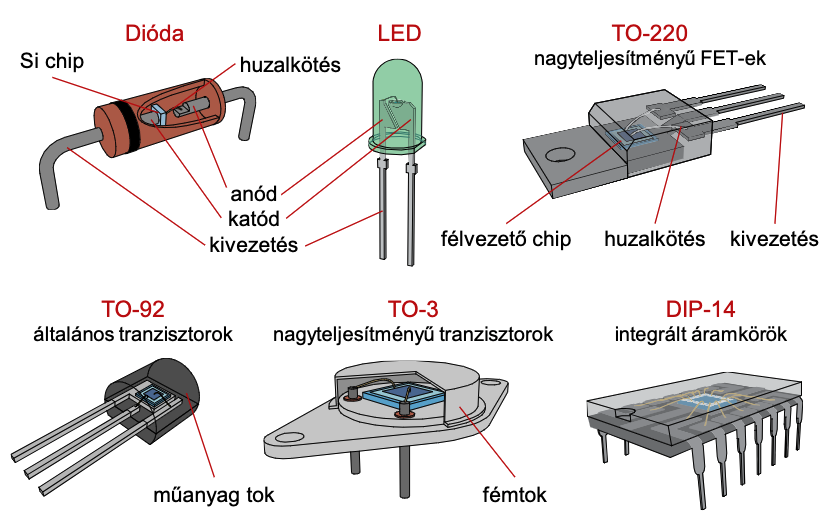
\includegraphics[width=.95\textwidth]{images/2.6/1.png}\end{center}

\end{document}